\documentclass{article}
\usepackage{amsfonts}
\usepackage[a4paper, total={7in, 10in}]{geometry}
\usepackage[dvipsnames]{xcolor}
\usepackage{fancyvrb}
\usepackage{graphicx}

\title{Report on Capstone Project:\\ Segmentation of houses for sale in Eau Claire, WI}
\author{Eric Canton}

\begin{document}
\maketitle

\section{Introduction: Business Problem}
A young professor couple are moving to Eau Claire, Wisconsin this summer, and want to buy a house. Eau Claire is a small ``college city'' focused around the University of Wisconsin, Eau Claire campus. There are numerous fairs and festivals in the summer, and avid crosscountry skiing and snowshoeing groups in the winters. 

This couple have generous moving funds from their new jobs, so they hire our realtor consulting firm specializing in finding young professionals homes they love in unfamiliar cities. We are the contracted consultants for these clients. Our goal is to provide our clients with an easy-to-use and -understand description of the housing market in Eau Claire. Interactive maps are familiar to most people these days, so we will present our findings to the clients in a Folium map; the locations we find will include links to the property listings, so they can use the websites we scrape to set up viewings of houses and hopefully close on their new home. 

\subsection{Guiding wishes from the clients}
\begin{enumerate}
\item The couple hope to have children soon, so definitely want to be near schools. 
\item They'd also like for there to be things in walking distance, like parks or
downtown areas, but don't want to live downtown.
\item They also want to be aware of local coffee shops where they can go to work remotely. 
\item Related to their wish to be able to walk places but not live downtown, we will evaluate the density of venues in the various regions of Eau Claire. 
\end{enumerate}

We close this section by noting that while the specific maps produced are mostly of interest to home-buyers looking to move to Eau Claire, WI, the ideas used here can easily be adapted to other locations and segmentation of house listings based on client preferences for venues they want to live near, like ``Korean and Italian restaurants'' or ``botanical gardens''. 

\section{Data Description}
After giving an overview of the data we need to perform our segmentation, we will expand some on the steps we use to collect this data. For more details, see the next section, Methodology. 

\subsection{Data: Overview}
The data we need is all related to locations in Eau Claire. 

First, we will need to get some listings
of houses for sale in the area; to make these most useful, we also want links to the listing, so that
our clients can pursue any houses that appeal to them, and we want to provide them with information 
about the listings like the number of bedrooms, bathrooms, and the price. 

Second, we will need information about venues around the houses we find. Since the couple want 
to have children, we'll look for schools (preschools, elementary, middle, and high schools), 
parks, and playgrounds. We will look for libraries and bookstores, both for their future kids
and because the clients are book lovers themselves. We will also search for coffee shops. Finally,
we will estimate the density of the immediate areas around the houses by counting the number
of venues within 750 meters. 

\subsection{Data: Collection}
Our general strategy will be to scrape house listing data off of Trulia.com and then make some
{\tt search} and {\tt explore} requests to the Foursquare API to get information about venues. More precisely:
\begin{enumerate}
\item We will use {\tt selenium.webdriver.Firefox}, running in headless mode, to get the HTML file for Eau Claire house listings on Trulia. These GET requests return 30 listings per page, so we'll get 2 pages. 
\item The page source we will pass through the BeautifulSoup {\tt html.parser} to aid our scraping of the contents of that page.
\item Using the {\tt find\_all(``a'')} method of our soup object, we can easily find the links within each page we downloaded in the first step. We filter the links by their text: house listing texts all end with ``WI'' (Wisconsin's state abbreviation), whereas the other links on the page have some other text. The {\tt find\_all} method returns a list of these tags and their associated content. Let's look at an example of one of these list elements. There is a lot of HTML describing how to display the little boxes for the houses, some images and alt-text, and so on, so we have pruned the output a bit here to highlight the tags we are most interested in. The original indentation has been preserved here, to give some sense of the nested depth of these tags. (BeautifulSoup makes simple work of extracting these tags!)
    \begin{Verbatim}[commandchars=\\\{\}]
     <a href="/p/wi/eau-claire/6708-timber-ln-eau-claire-wi-54701--2054962325">
   ...
   <span ... data-testid="property-tag-0">
    <span>
     {\color{red} NEW}
    </span>
   </span>
     ...
     <div ... data-testid="property-price">
      \textcolor{red}{$379,000}
     </div>
       ...
       <div ... data-testid="property-beds">
        {\color{red} 4bd}
       </div>
      ...
      </div>
       <div ... data-testid="property-baths">
        {\color{red} 3ba}
       </div>
      ...
       <div ... data-testid="property-floorSpace">
        {\color{red} 3,077 sqft}
       </div>
       ...
   <div ... data-testid="property-street">
    {\color{red} 6708 Timber Ln}
   </div>
   <div ... data-testid="property-region">
    {\color{red} Eau Claire, WI}
   </div>
    ...
     </a> 
\end{Verbatim}
        Suppose we have stored this {\tt find\_all} list element in the variable {\tt L}. Then {\tt L.text} would return the string:
        \begin{verbatim}
        NEW$379,0004bd3ba3,077 sqft6708 Timber LnEau Claire, WI
        \end{verbatim} so we can see that the information we're interested in, like price, beds, baths, square footage/size, can all be found in the link text. The address is also in there, but is more difficult  to parse because it's not as uniform (as we see from looking at other listings' text). However, it is easy enough to get just these address strings by calling {\tt L.find(``div'', \{``data-test-id'' : ``property-street''\})}. 
\item Once we have the info about each listing loaded into our Listing objects, we'll ask Foursquare for some local venue information. 
    \begin{itemize}
        \item Coffee shops
        \item Libraries
        \item Book stores
        \item Parks
        \item Schools
    \end{itemize}
\item Finally, we will pass some "explore" requests to Foursquare, using the response to investigate the areas with dense and sparse venues. These, along with the listings from the previous item,  will be used to rate the "venue density". 
\end{enumerate}

\section{Data: Reporting/Deliverable}
The primary means of presenting the gathered data to the client will be through two Folium maps. 
\begin{enumerate}
    \item The first map will have the Listing objects plotted, with HTML tags including the information from Listing member variables. These will be attached to CircleMarkers, colored according to segmentation formed via unsupervised DBSCAN, obtained from Scikit-Learn's OPTICS algorithm. On this map we will also plot the venues of interest mentioned before, color-coded based on their category; for example, the coffee shops will be shown as brown CircleMarkers on this map, and the libraries as teal CircleMarkers. 
    \item The second map will have the Listings plotted, colored according to the density of venues (of any kind) within 750 meters of the address. The density clustering will be done using $K$-means, with $K=3$. 
\end{enumerate}
The advantage of presenting the analysis of Eau Claire homes in this way is that the maps are interactive, and are a very familiar format based on pervasive use of websites like Google maps. 

\section{Methodology}
In this section, we expand on the steps we took to create the final product for our clients. 

\subsection{Importing packages}
The importing of packages/libraries we need is accomplished first. 
\begin{Verbatim}[commandchars=\\\{\}]
    {\color{JungleGreen}import} time
    {\color{JungleGreen}import} pickle

    {\color{JungleGreen}import} numpy {\color{JungleGreen}as} np
    {\color{JungleGreen}import} pandas {\color{JungleGreen}as} pd
    {\color{JungleGreen}import} matplotlib.pyplot {\color{JungleGreen}as} plt
    {\color{JungleGreen}import} matplotlib

    {\color{JungleGreen}from} sklearn.cluster {\color{JungleGreen}import} OPTICS, cluster_optics_dbscan, KMeans
    {\color{JungleGreen}from} sklearn.preprocessing {\color{JungleGreen}import} StandardScaler

    {\color{Gray}# Web stuff}
    {\color{JungleGreen}from} bs4 {\color{JungleGreen}import} BeautifulSoup
    {\color{JungleGreen}import} requests
    {\color{JungleGreen}from} selenium.webdriver {\color{JungleGreen}import} Firefox
    {\color{JungleGreen}from} selenium.webdriver.firefox.options {\color{JungleGreen}import} Options

    {\color{Gray}# Map stuff}
    {\color{JungleGreen}from} geopy.geocoders {\color{JungleGreen}import} Nominatim {\color{JungleGreen}as} Nom
    {\color{JungleGreen}import} folium
\end{Verbatim}
The {\tt pickle} package is used only to save the listings and venues we find for re-loading without re-downloading and scraping, which not only takes time due to API requirements (e.g., Nominatim restricts calls to 1 per second, accomplished using {\tt time}) and network availability/speed. 

\subsection{Python classes for Listing and Venue}
We created two Python classes, one called Listing and one called Venue, that store data associated to the houses and venues we find. These are defined as follows.
\begin{Verbatim}[commandchars=\\\{\}]
    {\color{JungleGreen}class} Listing:
        {\color{JungleGreen}def} __init__({\color{Cerulean}self}, addr : str, web : str, ll : tuple, parsed_link_text : tuple):
            {\color{Cerulean}self}.addr = addr
            {\color{Cerulean}self}.price, {\color{Cerulean}self}.beds, {\color{Cerulean}self}.bath, {\color{Cerulean}self}.sqft = parsed_link_text
            {\color{Cerulean}self}.web = web
            {\color{Cerulean}self}.ll = ll
            {\color{Cerulean}self}.venues = []

    {\color{JungleGreen}class} Venue:
        {\color{JungleGreen}def} __init__({\color{Cerulean}self}, name, cat = {\color{JungleGreen}None}, ll = {\color{JungleGreen}None}, web = {\color{JungleGreen}None}):
            {\color{Cerulean}self}.name = name
            {\color{Cerulean}self}.cat = cat
            {\color{Cerulean}self}.ll = ll
            {\color{Cerulean}self}.web = web
    
        {\color{JungleGreen}def} get_link({\color{Cerulean}self}):
            {\color{JungleGreen}return} "https://foursquare.com/v/" + {\color{Cerulean}self}.web
\end{Verbatim}
We populated Python lists of these classes, {\tt Ls} (for Listings) and {\tt key\_venues} (for Venues), during our scraping phase (described above in the Data section). These lists were used a number of times throughout our analysis and Folium map creation. 

\subsection{Machine Learning Techniques}
We used two machine learning techniques from Scikit-Learn: $K$-means clustering and OPTICS. %, DBSCAN, and a Decision Tree Classifier. 
\begin{itemize}
    \item We used $K$-means clustering ($K=3$) on the densities of nearby venues; the clusters we considered as high, medium, and low densities. We chose $K$-means clustering here because we had a definite goal of ending with 3 different clusters, and other unsupervised ML strategies like DBSCAN look for natural clusters, with no objective quantity of clusters.% Initially we tried to use OPTICS followed by DBSCAN, but we got more than 3 clusters and they were difficult to interpret, so went with the simpler $K$-means. 
    \item We used OPTICS for segmentation of the Listings we found based on the quantities of Schools, Coffee Shops, Libraries, Bookstores, and Parks/Playgrounds, within a 1.5 mile radius of each house listing. Before running our data through OPTICS, we first used the {\tt sklearn.preprocessing} Standard Normalizer, because some basic EDA revealed that there many parks and playgrounds in Eau Claire, and far fewer of some other kinds of venues, and we didn't want the Parks/Playgrounds category to dominate the segmentation. 

        We wanted to use DBSCAN because it allows for discovery of natural, arbitrarily shaped clusters within the data, and we had no preconcieved notions of the quantity of clusters we wanted, so $K$-means would not be an appropriate choice. However, DBSCAN has two main drawbacks:
        \begin{enumerate}
            \item the implementation of DBSCAN that Scikit-Learn uses is very expensive, both in terms of processor and RAM consumption. 
            \item any DBSCAN implementation necessitates specifying the $\varepsilon$ (epsilon) and $MinPts$ parameters to determine the minimum density to be used for clusters. 
        \end{enumerate}
        We instead used a kind of generalization of DBSCAN called OPTICS. While we still need to specify $MinPts$, no $\varepsilon$ parameter is needed and indeed one goal of this algorithm is to allow the user to discover clusters with a varying $\varepsilon$ (per cluster). This is done by evaluating the closeness of points in a specific order,  recording clusters by valleys in the so-called reachability distance. OPTICS also allows one to get around the processor and memory cost of running DBSCAN; while others' research shows OPTICS takes about 1.6 times as long, both implementations in Scikit-Learn currently run in $O(n^2)$. See the next section, Exploratory Data Analysis, for more information on this ranking and the ultimate clustering we found using the $\xi$-steepness method. 

%    \item We attempted to use a decision tree classifier to gain insight into the clustering found by the DBSCAN (after OPTICS). However, the resulting trees were too complicated to be very useful when the leaf nodes had high accuracy (low gini), and limiting the depth resulted in an insufficiently accurate tree. Ultimately, we decided not to include this tree in the deliverable to the client, nor in the polished Jupyter Notebook. A scaled-down version of the high-accuracy tree is shown below, to emphasize how complicated the this tree was. 
%        \begin{center}\includegraphics[scale=0.15]{tree.pdf} \end{center}
%        The coloring of the leaves corresponds to the coloring we used on our Folium maps, and is according to cluster. 
%
\end{itemize}

\subsection{Exploratory Data Analysis}

We used exploratory data analysis in two ways: to analyze the clusters resulting from $K$-means, and to choose the $\varepsilon$ (epsilon) parameter to use in our DBSCAN, based on the ``reachability graph'' produced from OPTICS. 
\vspace{1cm}

\noindent{\bf Analyzing $K$-means clustering.} Before fitting an instance of {\tt sklearn.cluster.KMeans(n\_clusters=3)} on our density data, we plotted the densities to estimate the clustering that we hoped to find. The densities were calculated on the number of venues $N$ returned using 
\begin{verbatim}GET https://api.foursquare.com/v2/venues/explore?...&radius=750&limit=50\end{verbatim}
dividing $N$ by 50. We notice there are two larger jumps, centered around densities 0.2 and 0.4, and indeed these were the break points that $K$-means ended with, too. 

\begin{minipage}{0.6\textwidth}
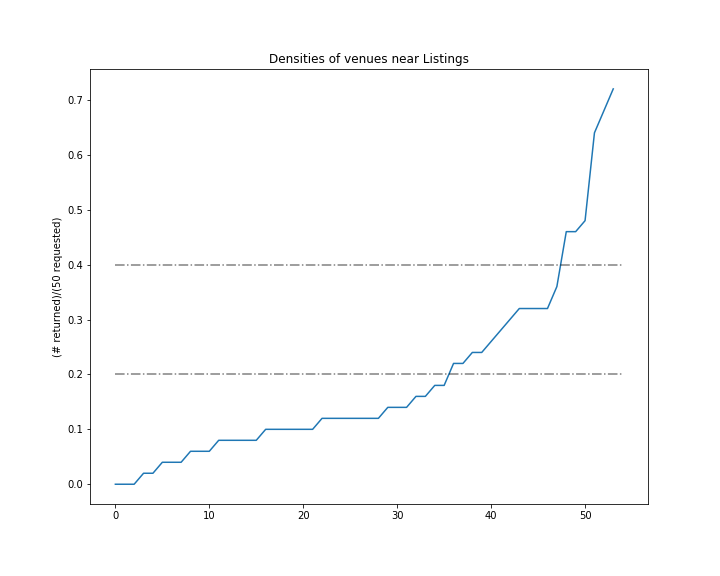
\includegraphics[scale=0.45]{Densities_plot.png}
\end{minipage}
\begin{minipage}{0.35\textwidth}
The densities ranged from 0 to 0.72; recall that we computed density out of 50 venues within 750 meters. The dashed lines correspond to break points in the clusters. More precisely, $K$-means gives:
\begin{verbatim}
======================
Density class: 0
Min: 0.0
Max: 0.18
======================
Density class: 1
Min: 0.22
Max: 0.36
======================
Density class: 2
Min: 0.46
Max: 0.72
======================
\end{verbatim}
\end{minipage}

\vspace{1cm}
\noindent{\bf Analyzing OPTICS reachability graph.} As hinted at in the previous subsection, OPTICS processes the points in a data set in a specific order and measures the so-called {\em reachability distance} from the current point under consideration to those already processed. This reachability distance essentially captures the radius $r$ one would have to use to cause the current point to be considered in the same cluster as the closest previous point. Thus, if we plot the reachability distances calculated in the order that OPTICS processes the points, then we can visually see the clusters as ``valleys'' in this reachability plot: remembering that the reachability distance $r(P_j)$ of the $j$-th considered point $P_j$ primarily involves $P_j$'s distance to $P_{j-1}$, we see that when the reachability drops it indicates that $P_j$ is much closer to $P_{j-1}$ than $P_{j-1}$ was to $P_{j-2}$, etc. 

%\footnote{Ankerst, Breuning, Kriegel, Sander. {\em OPTICS: Ordering Points To Identify the Clustering Structure.} Proc. ACM SIGMOD'99 Int. Conf. on Management of Data, Philadelphia, PA, 1999.}
The paper \footnote{Ankerst, Mihael, Markus M. Breunig, Hans-Peter Kriegel, and Jörg Sander. “OPTICS: ordering points to identify the clustering structure.” ACM SIGMOD Record 28, no. 2 (1999): 49-60.} originating the OPTICS algorithm proposed the so-called $\xi$-steepness clustering method, where cluster boundaries are identified on the reachability plots by finding regions where consecutive points are at least $\xi$\% greater or less than the points before. The advantage of this method is that it does not require a fixed threshold be used to decide on what makes a cluster, like one has to do with DBSCAN. 

\hspace{-2.5cm}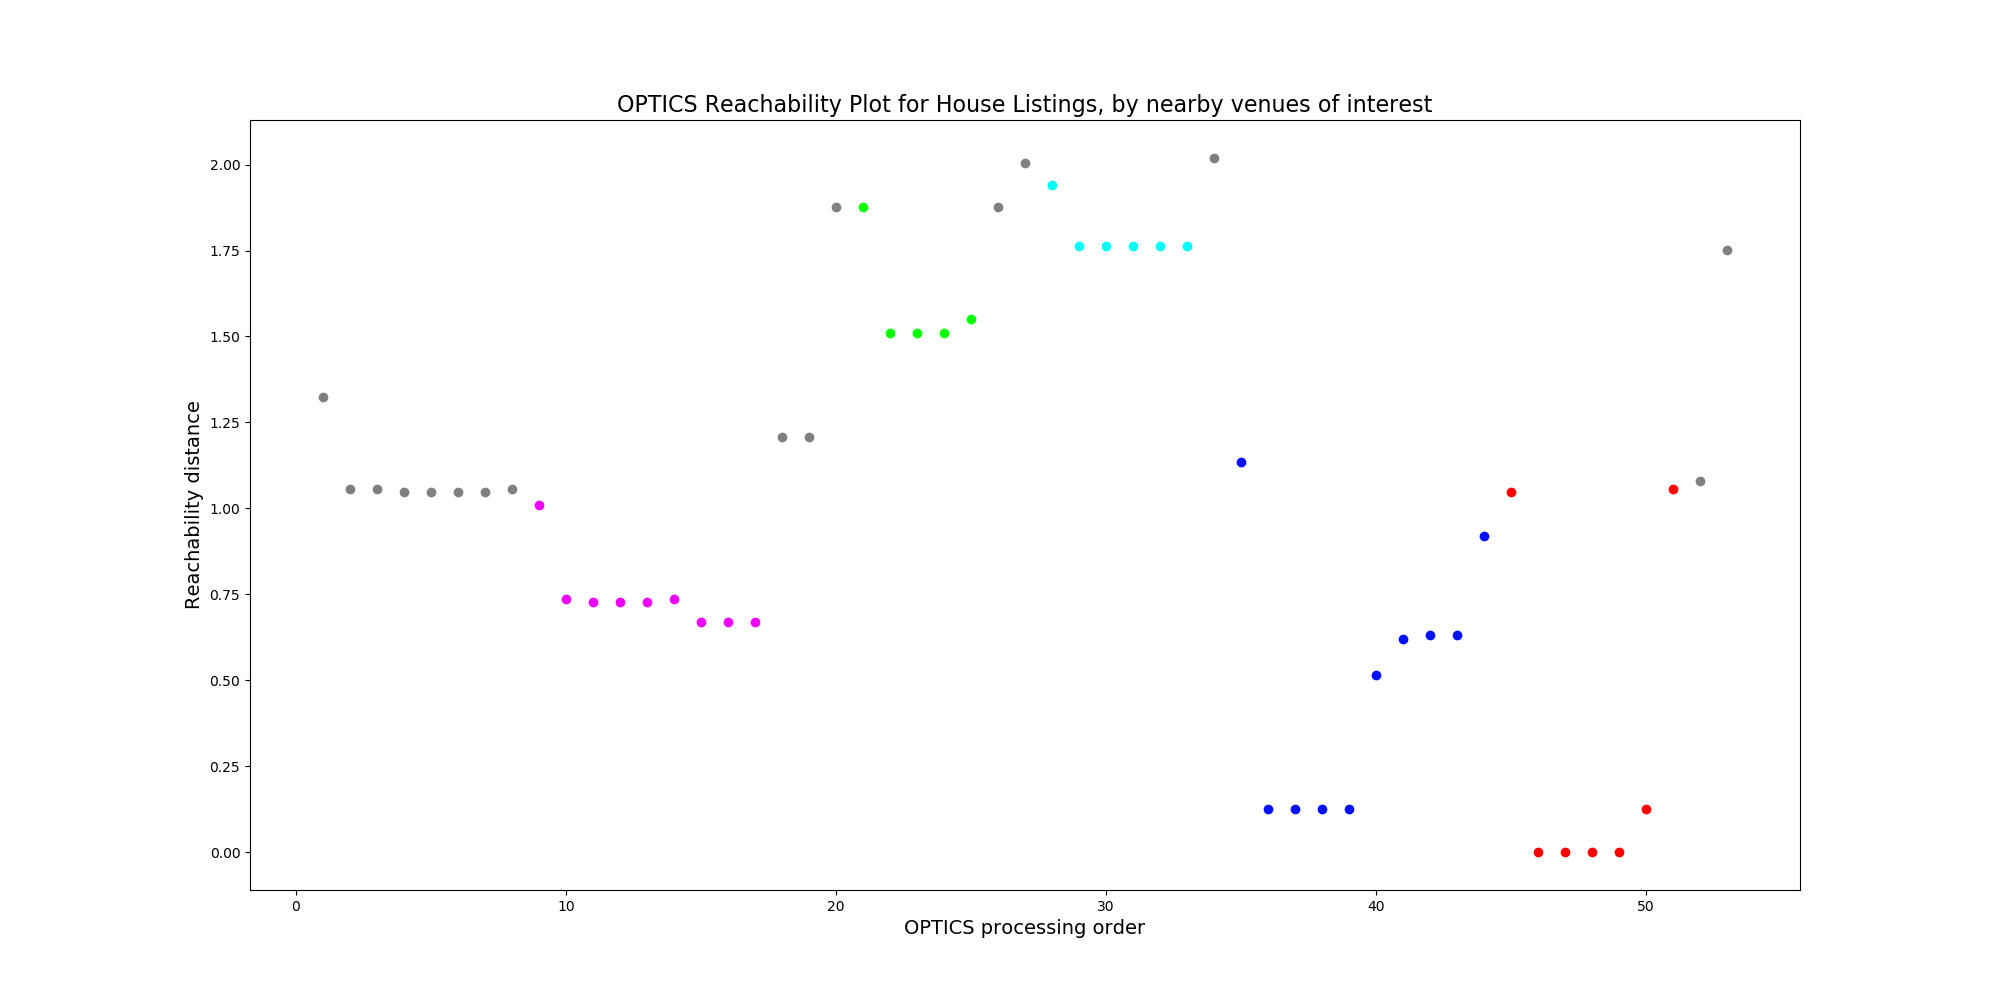
\includegraphics[scale=0.43]{OPTICS_reachability_2.png}

\section{Results and discussion}

Our analysis of the density of venues around house listings in Eau Claire, Wisconsin, indicate that in addition to the expected high densities near downtown and the university campus, there is another region where there are many stores southeast of the downtown area, near the mall. Once one leaves the downtown area, the density of stores decreases rapidly (aside from the mall). The houses are, however, seemingly evenly spread across the city and surrounding suburbs/exurbs. 

OPTICS revealed five natural clusters in the housing. In order to give some meaning to these clusters for our clients, we created a scatterplot with the OPTICS cluster on the $x$-axis and the average number of each type of venue (coffee shops, libraries, bookstores, parks/playgrounds, schools) within 1.5 miles of the listing. 

\hspace{-2.5cm}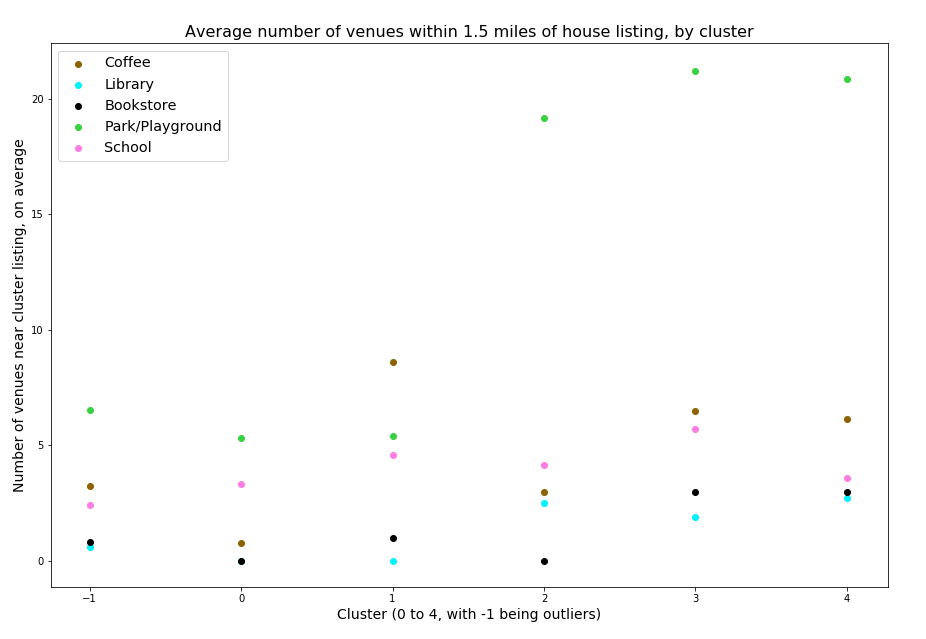
\includegraphics[scale=0.43]{Avg_venues.png}

This scatterplot reveals some interesting information about Eau Claire that is possibly difficult to get in other ways. For example, we see that there are between 3 and 7 schools near each of the listing clusters, on average. Additionally, there are two dramatically distinct groupings in terms of the average number of parks and playgrounds near the listings, with the outliers (group -1), and groups 0 and 1, having 5 to 7 parks nearby; the remaining clusters average 19 to 22 parks and playgrounds in the vicinity. The other features are more similar in terms of the average number of venues of each category nearby. Cluster 1 has the most coffee shops, on average, and looking at the below Folium maps we see that these are clustered around the aforementioned shopping center southeast of downtown. Some independent research shows that there are several small/local coffee shops in the downtown area, but seemingly not so close to the many listings in the {\em Third Ward} neighborhood (or at least not to be found on Foursquare by our methods).




\end{document}

